\documentclass{article}
\usepackage{xeCJK}
\setCJKmainfont[BoldFont=STHeiti, ItalicFont=STSong]{STSong}
\setCJKsansfont[BoldFont=STHeiti]{STXihei}
\setCJKmonofont{STFangsong}
\setmainfont{Times New Roman}
\usepackage{listings}
\usepackage{geometry}
\usepackage{minted}
\AtBeginEnvironment{minted}{%
	\renewcommand{\fcolorbox}[4][]{#4}}
\usepackage{graphicx}
\usepackage{color}   %May be necessary if you want to color links
\usepackage[hidelinks]{hyperref}
\hypersetup{
	colorlinks=false, %set true if you want colored links
	linktoc=all,     %set to all if you want both sections and subsections linked
	linkcolor=blue,  %choose some color if you want links to stand out
}

\geometry{a4paper,left=3.18cm,right=3.18cm,top=2.54cm,bottom=2.54cm}

\title{编译原理大作业实验报告}
\author{金连源、黄文璨、赵竟霖}

\begin{document}
	

\newpage
\tableofcontents
\newpage


\section{序言}

\quad \ \  我们实现的是一个类C语言的编译器,该语言包含了C语言的绝大部分特性,该编译器可以将C语言的代码转化成x86汇编指令。

组员的分工如下:
\begin{itemize}
\item 赵竟霖:代码生成和优化
\item 黄文璨:语义分析和错误处理
\item 金连源:词法分析和语法分析
\end{itemize}

\section{词法分析}

\subsection{简介}

\quad \ \  词法分析(英语:lexical analysis)是计算机科学中将字符序列转换为单词(Token)序列的过程。进行词法分析的程序或者函数叫作词法分析器(Lexical analyzer,简称Lexer),也叫扫描器(Scanner)。在本实验里面读取的大都是和C语言代码中相关的token,程序是用ply.lex实现的,它的底层原理是有限状态机。执行函数以后的返回结果是token的序列。

\subsection{实现细节}

\subsubsection{C语言关键字(keyword)}

\quad \ \  在ply.lex下,C语言的关键字必须单独的处理,不然会出现二义性的问题。
以下是编译器中关键字以及它的token表达形式:

\begin{itemize}
\item 'if' : 'IF'
\item 'else' : 'ELSE'
\item 'while' : 'WHILE'
\item 'return' : 'RETURN'
\item 'break' : 'BREAK'
\item 'void'  : 'VOID'
\item  'int'   : 'INT'
\item 'float' : 'FLOAT'
\item 'char'  : 'CHAR'
\item 'double' : 'DOUBLE'
\item 'struct' : 'STRUCT'
\item  'for' : 'FOR'
\item 'continue' : 'CONTINUE'
\item 'putchar' : 'PUTCHAR'
\item 'getchar' : 'GETCHAR'
\end{itemize}

\subsubsection{C语言其他符号}

\quad \ \  除了关键字以外,我们还需要处理C语言其他的符号,下面列出它们所表达的含义以及它们所对应的正则表达式:

\begin{table}[H]
	%\caption{l\_orderkey comparison}
	\centering
	\begin{tabular}{|c|c|c|c|c|c|c|}
		\hline
		\bf token  				& \bf 解释	      & \bf 正则表达式      \\\hline
		PLUS 	 				 & 加号		  & r'+'    \\\hline
		MINUS     				& 减号  &  r'-'    \\\hline
		TIMES 	 				 & 乘号		  & r'*'    \\\hline
		DIVIDE     				 & 除号  &   r'/'  \\\hline
		DOUBLEPLUS 	 	& 加加		  &  r'++'   \\\hline
		DOUBLEMINUS     & 减减  &   r'--'    \\\hline
		PLUSEQUAL 	 	 & 加等于		  & r'+='   \\\hline
		MINUSEQUAL     & 减等于  &  r'-='   \\\hline
		TIMESEQUAL 	 	& 乘等于		  & r'*='   \\\hline
		DIVIDEEQUAL     & 除等于  &  r'/='    \\\hline
		SINGLEEQUAL 	 	& 赋值		  & r'='   \\\hline
		DOUBLEEQUAL     & 等于判断  &   r'=='  \\\hline
		DOUBLEPIPES 	 	& 或运算		  &r'||'    \\\hline
		DOUBLEAMPERSAND     & 与运算  &  r'\&\&'   \\\hline
		BANGEQUAL 	 					& 不等于		  & r'!='    \\\hline
		LPAREN     				& 左圆括号  &  r'('    \\\hline		
		RPAREN 	 	& 右圆括号		  & r')'    \\\hline
		LCURLY     & 左大括号  &  r'\{'    \\\hline
		RCURLY 	 	& 右大括号		  & r'\}'    \\\hline
		LSQUARE     & 左方括号  &   r'['  \\\hline
		RSQUARE 	 	& 右方括号		  & r']'    \\\hline
		SEMICOLON     & 分号  &  r';'    \\\hline
		COMMA 	 	& 逗号		  & r','    \\\hline
		ID     & 标识符  &  r'[a-zA-Z\_][a-zA-Z\_0-9]*''    \\\hline
		LANGLE 	 	& 小于符号		  & r'<'    \\\hline
		RANGLE     & 大于符号  &  r'>'    \\\hline
		LANGLEEQUAL 	 	& 小于等于		  & r'<='    \\\hline
		RANGLEEQUAL     & 大于等于  &   r'>='  \\\hline
		EXCLAMATION     & 感叹号  &   r'!'  \\\hline
		PERCENT 	 	& 	百分号	  & r'\%'    \\\hline
		DOT     & 点运算符  &  r'.'    \\\hline
		ADDR 	 	& 取地址符		  & r'\&'    \\\hline
		LEFTARROW     & 箭头符号  &  r'->'    \\\hline
		FLOATLITERAL 	 	& 浮点数值		  & r'$\backslash$d+.$\backslash$d+'    \\\hline
		INTLITERAL     & 整数值  &  r'$\backslash$d+'    \\\hline
		STRINGLITERAL 	 	& 字符串值		  & r'$\backslash$ " ($\backslash$ . | [ $\backslash$ \^ $\backslash$ "])*$\backslash$"'   \\\hline
	\end{tabular}
\end{table}


\subsection{测试结果}

考虑如下C语言代码

\begin{minted}{c}
int f;
int k;

int go(int* b, int a)
{
    int fk;
    double t;
    int g;
    if(a > 0){
        g = a * go(b, a-1);
    }else{
        g = 1;
    }
    *b = *b + g;
    k = k + g;
    return g;
}

int main(void)
{
    k = 0;
    f = go(&k, 5);
    printf("%d\n", f);
    printf("%d\n", k);
    return 0;
}
\end{minted}

它的对应的token序列如下:

\begin{minted}{shell}
LexToken(INT,'int',2,1)
LexToken(ID,'f',2,5)
LexToken(SEMICOLON,';',2,6)
LexToken(INT,'int',3,8)
LexToken(ID,'k',3,12)
LexToken(SEMICOLON,';',3,13)
LexToken(INT,'int',5,16)
LexToken(ID,'go',5,20)
LexToken(LPAREN,'(',5,22)
LexToken(INT,'int',5,23)
LexToken(TIMES,'*',5,26)
LexToken(ID,'b',5,28)
LexToken(COMMA,',',5,29)
LexToken(INT,'int',5,31)
LexToken(ID,'a',5,35)
LexToken(RPAREN,')',5,36)
LexToken(LCURLY,'{',6,38)
LexToken(INT,'int',7,44)
LexToken(ID,'fk',7,48)
LexToken(SEMICOLON,';',7,50)
LexToken(DOUBLE,'double',8,56)
LexToken(ID,'t',8,63)
LexToken(SEMICOLON,';',8,64)
LexToken(INT,'int',9,70)
LexToken(ID,'g',9,74)
LexToken(SEMICOLON,';',9,75)
LexToken(IF,'if',10,81)
LexToken(LPAREN,'(',10,83)
LexToken(ID,'a',10,84)
LexToken(RANGLE,'>',10,86)
LexToken(INTLITERAL,0,10,88)
LexToken(RPAREN,')',10,89)
LexToken(LCURLY,'{',10,90)
LexToken(ID,'g',11,100)
LexToken(SINGLEEQUAL,'=',11,102)
LexToken(ID,'a',11,104)
LexToken(TIMES,'*',11,106)
LexToken(ID,'go',11,108)
LexToken(LPAREN,'(',11,110)
LexToken(ID,'b',11,111)
LexToken(COMMA,',',11,112)
LexToken(ID,'a',11,114)
LexToken(MINUS,'-',11,115)
LexToken(INTLITERAL,1,11,116)
LexToken(RPAREN,')',11,117)
LexToken(SEMICOLON,';',11,118)
LexToken(RCURLY,'}',12,124)
LexToken(ELSE,'else',12,125)
LexToken(LCURLY,'{',12,129)
LexToken(ID,'g',13,139)
LexToken(SINGLEEQUAL,'=',13,141)
LexToken(INTLITERAL,1,13,143)
LexToken(SEMICOLON,';',13,144)
LexToken(RCURLY,'}',14,150)
LexToken(TIMES,'*',15,156)
LexToken(ID,'b',15,157)
LexToken(SINGLEEQUAL,'=',15,159)
LexToken(TIMES,'*',15,161)
LexToken(ID,'b',15,162)
LexToken(PLUS,'+',15,164)
LexToken(ID,'g',15,166)
LexToken(SEMICOLON,';',15,167)
LexToken(ID,'k',16,173)
LexToken(SINGLEEQUAL,'=',16,175)
LexToken(ID,'k',16,177)
LexToken(PLUS,'+',16,179)
LexToken(ID,'g',16,181)
LexToken(SEMICOLON,';',16,182)
LexToken(RETURN,'return',17,188)
LexToken(ID,'g',17,195)
LexToken(SEMICOLON,';',17,196)
LexToken(RCURLY,'}',18,198)
LexToken(INT,'int',20,201)
LexToken(ID,'main',20,205)
LexToken(LPAREN,'(',20,209)
LexToken(VOID,'void',20,210)
LexToken(RPAREN,')',20,214)
LexToken(LCURLY,'{',21,216)
LexToken(ID,'k',22,222)
LexToken(SINGLEEQUAL,'=',22,224)
LexToken(INTLITERAL,0,22,226)
LexToken(SEMICOLON,';',22,227)
LexToken(ID,'f',23,233)
LexToken(SINGLEEQUAL,'=',23,235)
LexToken(ID,'go',23,237)
LexToken(LPAREN,'(',23,239)
LexToken(ADDR,'&',23,240)
LexToken(ID,'k',23,241)
LexToken(COMMA,',',23,242)
LexToken(INTLITERAL,5,23,244)
LexToken(RPAREN,')',23,245)
LexToken(SEMICOLON,';',23,246)
LexToken(ID,'printf',24,252)
LexToken(LPAREN,'(',24,258)
LexToken(STRINGLITERAL,'"%d\n"',24,259)
LexToken(COMMA,',',24,264)
LexToken(ID,'f',24,266)
LexToken(RPAREN,')',24,267)
LexToken(SEMICOLON,';',24,268)
LexToken(ID,'printf',25,274)
LexToken(LPAREN,'(',25,280)
LexToken(STRINGLITERAL,'"%d\n"',25,281)
LexToken(COMMA,',',25,286)
LexToken(ID,'k',25,288)
LexToken(RPAREN,')',25,289)
LexToken(SEMICOLON,';',25,290)
LexToken(RETURN,'return',26,296)
LexToken(INTLITERAL,0,26,303)
LexToken(SEMICOLON,';',26,304)
LexToken(RCURLY,'}',27,306)
\end{minted}

\section{语法分析}

\subsection{简介}

语法分析是编译过程的一个逻辑阶段。语法分析的任务是在词法分析的基础上将单词序列组合成各类语法短语,如“程序”,“语句”,“表达式”等等.语法分析程序判断源程序在结构上是否正确.源程序的结构由上下文无关文法描述.语法分析程序可以用YACC等工具自动生成。在本实验中我们使用了ply.yacc的语法分析工具,采用的算法是LAIR(1)。程序执行的结果是一棵语法树,由python数据结构里的元组和列表来表示。

\subsection{实现细节}

\quad \ \ 我们实现的minic语言实现了C语言的大多数语法,不过出于简便,我们对C语言的语言规则进行了一定的限制。以下是我们的一些文法规则和解释:
\begin{minted}{shell}

program : declarationList
declarationList : declarationList declaration
                | declaration
declaration : staticVariableDeclaration
            | functionDeclaration

\end{minted}

解释:在这里program是整一份代码的顶端入口,这是一个最顶层的文法规则。在这里声明列表是由一系列的声明所构成的,全局下的声明又是由函数和全局变量声明所构成的。

\begin{minted}{shell}
functionDeclaration : typeSpec ID LPAREN parameters RPAREN compoundStatement

typeSpec            : VOID
                    | INT
                    | FLOAT
                    | CHAR
                    | DOUBLE
                    | structSpecifier
                              
structSpecifier     : STRUCT ID LCURLY staticVariableDeclarationList RCURLY
                    | STRUCT ID
\end{minted}

解释:函数声明的文法如上所示,typeSepc是函数的返回类型,ID是函数的名字,parameters是参数的列表,compoundStatement是函数体。

\begin{minted}{shell}

compoundStatement : LCURLY optionalLocalDeclarations optionalStatementList RCURLY

whileStatement : WHILE LPAREN expression RPAREN statement

forStatement : FOR LPAREN optionalExpression SEMICOLON optionalExpression SEMICOLON 
optionalExpression RPAREN statement

breakStatement : BREAK SEMICOLON

ifStatement : IF LPAREN expression RPAREN statement optionalElseStatement

returnStatement : RETURN expression SEMICOLON

continueStatement : CONTINUE SEMICOLON

\end{minted}

解释:块语句的定义如上所示,在大括号里面包含了局部变量的声明以及局部逻辑控制语句。在这里列出我们实现的主要逻辑控制语句,分别是:if条件判断语句、for循环语句、while循环语句、break语句、continue语句和return语句。

\begin{minted}{shell}
staticVariableDeclaration : typeSpec declaratorList SEMICOLON
                          | typeSpec declarator LSQUARE INTLITERAL RSQUARE SEMICOLON

declarator : pointer ID
           | ID

pointer : TIMES
        | TIMES pointer
\end{minted}

解释:以上是静态变量声明的语句,这里的静态变量包含了不同变量的声明和数组的声明,出于简便起见我们的数组只允许单独声明,不能和普通变量出现在一个声明语句以内。我们同时也实现了指针的声明。

\begin{minted}{python}
precedence = (
#('nonassoc','LESSTHAN', 'GREATERTHAN'),
('right','SINGLEEQUAL','PLUSEQUAL','MINUSEQUAL','DIVIDEEQUAL','TIMESEQUAL'),
('left', 'DOUBLEPIPES'),
('left', 'DOUBLEAMPERSAND'),
('left','BANGEQUAL','DOUBLEEQUAL'),
('left', 'LANGLE','RANGLE','LANGLEEQUAL','RANGLEEQUAL'),
('left', 'PLUS', 'MINUS'),
('left', 'TIMES', 'DIVIDE', 'PERCENT'),
('left', 'LSQUARE'),
('right', 'UMINUS','EXCLAMATION','REMOVEREF','ADDR'),
('left','ELSE')
)
\end{minted}

解释:由于expression的定义较为复杂,我们首先确定了它的优先级以及结合的顺序

\begin{minted}{shell}

expression : expression PLUS expression
           | expression MINUS expression
           | expression TIMES expression
           | expression DIVIDE expression
           | expression DOUBLEPIPES expression
           | expression DOUBLEAMPERSAND expression
           | expression LANGLE expression
           | expression RANGLE expression
           | expression LANGLEEQUAL expression
           | expression RANGLEEQUAL expression
           | expression BANGEQUAL expression
           | expression DOUBLEEQUAL expression
           | expression PERCENT expression
           
\end{minted}

解释:上面是二元运算表达式的文法,我们在这里实现了加、减、乘、除等基本的二元运算。

\begin{minted}{shell}
expression : expression DOT ID
expression : expression LEFTARROW ID
expression : ADDR expression
expression : REMOVEREF expression
\end{minted}

解释:以上是和指针以及结构体相关的文法,在这里我们实现了取地址、解引用的运算,并且实现了结构体变量以及结构体指针访问成员的运算。

\begin{minted}{shell}
expression : expression DIVIDEEQUAL expression
           | expression PLUSEQUAL expression
           | expression MINUSEQUAL expression
           | expression TIMESEQUAL expression

expression : expression DOUBLEPLUS
           | expression DOUBLEMINUS
\end{minted}

解释:以上是基于C语言特性的运算表达式,这里实现了加等于、减等于之类的压缩表示运算以及自加和自减的运算。

\subsection{测试结果}

考虑如下C语言代码:

\begin{minted}{c}
int ans;

int gcd(int a, int b)
{
    int g;
   if(b==0){
        g = a;
    }else{
        g = gcd(b, a % b);
    }
    return g;
}

int main(void)
{
    ans = gcd(9, 36) * gcd(3, 6);
    printf("%d\n", ans);
    return 0;
}
\end{minted}

它的语法结构在python的表达如下:

\begin{minted}{python}
('program', ('declarationList', [('declaration', ('staticVariableDeclaration',
('typeSpec', 'int'), ('declaratorList', [('declarator', 'ans')]))),
('declaration', ('functionDeclaration', ('typeSpec', 'int'), 'gcd', 
('parameters', ('parameterList', [('parameter', ('typeSpec', 'int'), 
('declarator', 'a')), ('parameter', ('typeSpec', 'int'), ('declarator', 'b'))])), 
('compoundStatement', ('optionalLocalDeclarations', ('localDeclarations', 
[('localDeclaration', ('staticVariableDeclaration', ('typeSpec', 'int'), 
('declaratorList', [('declarator', 'g')])))])), ('optionalStatementList', 
('statementList', [('statement', ('ifStatement', ('binary-expression', '==', 
('identifier-expression', 'b'), ('int-expression', 0)), ('statement', 
('compoundStatement', ('optionalLocalDeclarations', None), 
('optionalStatementList', ('statementList', [('statement', ('expressionStatement', 
('assignExpression', ('identifier-expression', 'g'), ('identifier-expression', 
'a'))))])))), ('optionalElseStatement', ('statement', ('compoundStatement', 
('optionalLocalDeclarations', None), ('optionalStatementList', ('statementList', 
[('statement', ('expressionStatement', ('assignExpression', 
('identifier-expression', 'g'), ('functioncallExpression', 'gcd', 
('argumentExpressionList', [('identifier-expression', 'b'), ('binary-expression', 
'%', ('identifier-expression', 'a'), ('identifier-expression', 'b'))])))))]))))))), 
('statement', ('returnStatement', ('identifier-expression', 'g')))]))))), 
('declaration', ('functionDeclaration', ('typeSpec', 'int'), 'main', ('parameters', 
'void'), ('compoundStatement', ('optionalLocalDeclarations', None), 
('optionalStatementList', ('statementList', [('statement', ('expressionStatement', 
('assignExpression', ('identifier-expression', 'ans'), ('binary-expression', '*', 
('functioncallExpression', 'gcd', ('argumentExpressionList', [('int-expression', 9), 
('int-expression', 36)])), ('functioncallExpression', 'gcd', ('argumentExpressionList', 
[('int-expression', 3), ('int-expression', 6)])))))), ('statement', ('expressionStatement', 
('functioncallExpression', 'printf', ('argumentExpressionList', 
[('stringExpression', '"%d\n"'), ('identifier-expression', 'ans')])))), 
('statement', ('returnStatement', ('int-expression', 0)))])))))]))

\end{minted}

\section{语义分析}

\subsection{简介}

\quad\ \ 语义分析是编译过程的一个逻辑阶段,语义分析的任务是对结构上正确的源程序进行上下文有关性质的审查,进行类型审查。语义分析是审查源程序有无语义错误,为代码生成阶段收集类型信息。比如语义分析的一个工作是进行类型审查,审查每个算符是否具有语言规范允许的运算对象,当不符合语言规范时,编译程序应报告错误。如有的编译程序要对实数用作数组下标的情况报告错误。又比如某些程序规定运算对象可被强制,那么当二目运算施于一整型和一实型对象时,编译程序应将整型转换为实型而不能认为是源程序的错误。


我们没有特别进行繁多的类型审查处理,而是只支持整数int类型的算数操作。我们实现的语义分析主要是为中间代码生成做准备工作,包括语法树的语义层面的解析和符号表的维护。


我们采用了语义分析和中间代码生成同时进行的方法,这里只介绍语义分析的基本方法和实现细节。

\subsection{基本方法}

\quad\ \ 将语法树按语句类型逐级分层,利用函数调用栈递归解析。

(1)例如下面分析语句的函数,根据语法树不同语句的语法规则,按类型分为:

if语句、表达式语句、函数返回语句、for语句、while语句、复合语句、break语句、continue语句等

并分别调用不同的解析函数完成递归解析。

\begin{minted}{python}
def parse_statement(statement,label_start="continue???",label_end="break???"):
       assert(statement[0]=="statement")
       assert(len(statement)==2)
       if statement[1][0]=="ifStatement":
            parse_ifstatement(statement[1],label_start,label_end)
       elif statement[1][0]=="expressionStatement":
            ret_temp_var(parse_expressionStatement(statement[1]))
       elif statement[1][0]=="returnStatement":
            parse_returnStatement(statement[1])
       elif statement[1][0]=="forStatement":
            parse_forStatement(statement[1])
       elif statement[1][0]=="whileStatement":
            parse_whileStatement(statement[1])
       elif statement[1][0]=="compoundStatement":
            parse_compoundStatement(statement[1],label_start,label_end)
       elif statement[1]=="breakStatement":
            print("\t"+str(("j",None,None,label_end)))
       elif statement[1]=="continueStatement":
            print("\t"+str(("j",None,None,label_begin)))
       else:
            print(statement[1])
            assert(False)
       return
\end{minted}

(2)又有如下关于解析声明的函数,按声明的类型分为:

函数声明、静态变量声明、静态变量数组声明等

然后递归调用不同的解析处理函数完成解析。

\begin{minted}{python}
def parse_declaration(declaration):
       assert(declaration[0]=="declaration")
       if declaration[1][0]=="functionDeclaration":
             parse_functionDeclaration(declaration[1])
       elif declaration[1][0]=="staticVariableDeclaration":
             parse_staticVariableDeclaration(declaration[1])
       elif declaration[1][0]=="staticVariableArrayDeclaration":
             parse_staticVariableArrayDeclaration(declaration[1])
       else:
             assert(False)
\end{minted}

\subsection{实现细节}

\quad\ \ 具体实现上,在递归调用解析函数的过程中对语句的主要信息解析记录和分析,以静态变量的声明为例:

当遇到一条如下c代码时,语法分析器会生成包含"int a;"声明的声明表declaration list。

\begin{minted}{C}
int a;
\end{minted}

语义分析器(即与中间代码生成器整合在一起的工具)按照如下处理栈对其进行分析。

\begin{minted}{python}
parse_declarationList ->
parse_declaration ->
parse_staticVariableDeclaration
\end{minted}

最后在parse\_staticVariableDeclaration函数中将该静态变量记录在全局变量符号表global\_var中。

\begin{minted}{python}
def parse_staticVariableDeclaration(staticVariableDeclaration):
       # ...
       global global_var
       var_type=staticVariableDeclaration[1][1]
       for _ in staticVariableDeclaration[2][1]:
             if len(_)==2:
                  global_var.append((var_type,_[1],(False,1),None))  # int a
             else:  # pointer
                   global_var.append((var_type+_[1][1][0],_[2],(False,1),None))
                     # int *a
       return
\end{minted}

\subsection{测试结果}

\section{符号表设计}

\subsection{简介}

\quad\ \    主要维护了两类符号,全局变量global\_var,和函数中的局部变量。函数中的局部变量又分为函数参数local\_para和函数内定义的变量local\_var。全局定义的函数又作为一种全局的函数变量。

由于我们采用的是,符号表与中间代码一起生成的方法。在此文档中仅介绍符号表生成的部分。

\subsection{实现细节}

\quad \ \ (1)采用Python字典数据结构dict存储符号表symbol\_table。
\begin{minted}{python}
symbol_table = {}
\end{minted}


(2)在分析declarationList之后得到全局变量,将其存储到符号表中
\begin{minted}{python}
def parse_declarationList(declarationList):
       assert(declarationList[0]=="declarationList")
       for _ in declarationList[1]:
             parse_declaration(_)
       global global_var
       print("global_var =",global_var)
       global symbol_table
       symbol_table.setdefault('global', {}).setdefault('global_var', global_var)
\end{minted}


(3)在分析函数参数时,将参数符号存储到符号表
\begin{minted}{python}
def parse_parameters(parameters, label_func):
       # ...
       parse_parameterList(parameters[1])
       # ...
       global symbol_table
       symbol_table.setdefault(label_func, {}).setdefault('local_para', local_para)
\end{minted}

(4)在分析函数定义之后得到函数内定义的局部变量,将其存储到符号表
\begin{minted}{python}
def parse_functionDeclaration(functionDeclaration):#1-> return type 2->name 3->para 4->body
# ...
       parse_parameters(functionDeclaration[3], label_func)
       assert(functionDeclaration[4][0]=="compoundStatement")
# ...
       global symbol_table
       symbol_table.setdefault(label_func, {}).setdefault('local_var', local_var)
\end{minted}

\section{代码生成}

\subsection{中间代码生成}

生成的中间代码是自定义的四元式,形如`(op,src1,src2,dest)`

\subsubsection{四元式}

\quad\ \ 四元式内容说明

\begin{itemize}
	\item  \textbf{op}说明指令的大致运算类型,它可以是某个双目运算符,或是某种赋值运算符,也可以是跳转指令,还可以是一些函数相关的汇编指令,如"call"(表示调用),"arg"(表示函数参数压栈),"ret"(表示函数返回);
	\item \textbf{src}说明操作数,它可以某个变量,或是某个常数,还可以是常数名字,特定情况下可以为空; 
	\item \textbf{dest}说明的是操作的目标,通常是一个变量或是变量组(用于说明给数组元素赋值),也可以是标签(用于跳转),特定情况下可以为空.
\end{itemize}

四元式中的作为操作数的变量不仅仅只有变量名这一个信息,而是作为一个元组,还带有额外信息用于辅助生成汇编代码.

操作数形如`(var\_name,(is\_global\_or\_temp,type,byte\_addr))`

其中:

\begin{itemize}
\item  \textbf{var\_name}是一个简单python字符串用以说明的变量名字,实际上在生成汇编的过程中只有使用全局变量时才会用到这个信息;
\item   \textbf{is\_global\_or\_temp}标记变量是否是全局变量或是局部的临时变量,取值为\textbf{True}或\textbf{False},或是一串python的bytes(说明是字符串);
\item  \textbf{type}是一个简单python字符串用以说明的变量类型,如"\textbf{int}", "\textbf{int*}", "\textbf{double}", "\textbf{char}", "\textbf{float}"等;
\item  \textbf{byte\_addr}指的是变量的偏移,不过参考的基准略有不同:\begin{itemize}
				\item  普通全局变量无意义,设为None
				\item  字符串常量,
				\item  函数局部参数,设置为相对于"\textbf{返回地址}"(\textbf{return address})的偏移(所以是非负数)
				\item  局部变量(非临时变量),相对于帧指针\textbf{ebp}的偏移地址(所以是负数)
				\item  局部变量(临时变量),相对于函数在栈中挖出当前函数所有变量空间后的栈指针\textbf{esp}的偏移地址(所以是正数)
				\end{itemize}
\end{itemize}

下方对若干自定义四元式举例说明:

\begin{minted}{python}
;i=0;给局部变量i赋值0,i的基地址在[ebp-44],数据宽度是sizeof(int)=4
(':=', 0, None, ('i', (False, 'int', -44)))

;temp_var_4=(i<10);其中temp_var_4是临时变量,假设函数所有变量的大小为x(Byte),
那么temp_var_4基地址为[ebp-x+0],数据宽度是sizeof(int)=4
('<', ('i', (False, 'int', -44)), 10, ('temp_var_4', (True, 'int', 0)))

;if(temp_var_4==0)goto main_L2;其中main_L2是一个标签
('j==', ('temp_var_4', (True, 'int', 0)), 0, 'main_L2')

;参数aFDDN的地址压栈
('arg', ('aFDDN', (b'"f[%d]=%d\\n"', 'char[]', 13)), None, None)

;调用函数printf;已经实现将参数压栈,printf的返回值实际上是成功输出的字符个数,
返回值最终存入temp_var_4
('call', 'printf', None, ('temp_var_4', (True, 'int', 0)))

;temp_var_4=&k;k是全局变量数据类型是int,temp_var_4是临时变量,数据类型int
(':=(&)', ('k', (True, 'int', None)), None, ('temp_var_4', (True, 'int', 0)))

;return g;其中g是局部变量,实际地址为[ebp-4],数据宽度sizeof(int)=4
('ret', ('g', (False, 'int', -4)), None, None)
\end{minted}

\subsubsection{函数调用}

\quad\ \ 这里特殊列出来是因为两个原因:

\begin{itemize}
\item 函数调用的时候有个针对字符串常量的特殊处理
\item 函数调用协议有很多种:\textbf{\_\_stdcall},\textbf{\_\_cdecl},"\textbf{\_\_pascall}","\textbf{\_\_thiscall}"以及\textbf{\_\_fastcall},实现函数调用在默认情况下必须统一为其中某一种.
\end{itemize}

\paragraph{函数调用中的字符串常量\\}
考虑这样一个代码

\begin{minted}{c}
printf("helloworld\n");
\end{minted}

在函数调用的过程中,正常的编译器不会把整个字符串压入堆栈(,除非setbuf清空了特定缓冲区),而是仅仅压入字符串的地址.但是为什么某个地址会恰好有这个字符串呢?答案就是,编译器在数据段(全局变量区域)有意构造了这样的字符串.


但是给这个字符串取名字也有点问题,毕竟最终的代码我们并不在意它的名字,但是在写汇编的过程中我们需要用符号助记它的基地址,这个名字又不能和其他全局变量重名...最终是参考了\textbf{IDA Pro}逆向可执行文件的时候给字符串命名的方式,自己设计了一个命名机制.


这个串会导致在数据段额外增加一些数据:

\begin{minted}{asm}
data segment
        aHELLOWORLDN "helloworld",0ah,0dh,0,'$'
data ends
\end{minted}

由于汇编没有字符串转移,表示"$\backslash$n"这个回车字符实际上将其转化为ascii码0ah就行了.至于后面还有0dh,这是因为Windows中,"\\n"实际上是执行了\textbf{回车(光标移到所在行行首)}和\textbf{换行(光标下移一位)}两个操作.再后面的0是c/c++字符串的结束标志.再在之后的'\$'是dos模式下字符的结束标志,放在这里是为了一定程度上避免被解释为dos下的exe运行的时候会出大问题.


函数真正调用的时候会被编译成:

\begin{minted}{asm}
push offset [aHELLOWORLDN]
call crt_printf;msvcrt.lib库的printf就叫这个名字
\end{minted}


\paragraph{函数调用协议\\}

调用协议的区别在网上有很多阐释,此处着重说明我们使用的\textbf{\_\_stdcall}

\begin{itemize}
\item 参数只能通过堆栈传递,进入函数时不会有寄存器储存参数;
\item 函数的压栈顺序是从右到左的;
\item  函数结束后,被调用者负责清理栈空间(函数参数占据的栈空间).
\end{itemize}

前面两个比较好理解,关于最后一个,一两份代码进行说明:
\textbf{被调用者负责清理栈空间示例}

\begin{minted}{asm}
code segment
f proc
       push ebp
       mov ebp,esp 
       mov eax,[ebp+8]
       inc eax
       mov esp,ebp
       pop ebp
       ret 4
f endp
main proc
       push ebp
       mov ebp,esp
       xor eax,eax
       push eax
       call f
       mov esp,ebp
       pop ebp
main endp
code ends
end main
\end{minted}

可以看到,被调用者清理栈空间,f函数最后是用`ret 4`返回的,说明找到返回地址之后,堆栈还得弹出4B的空间再返回.
与之相对的,调用者清理栈空间,f函数最后是用`ret`返回的,找到返回地址直接跳转.在main函数的call之后,还好有一个恢复堆栈的add指令.

由于\textbf{\_\_stdcall}适用于Win API, 我们就延续此传统使用了\textbf{\_\_stdcall}.

\subsubsection{变量定义(符号表)}

\quad\ \ 由于全局变量能在函数体以外的任何地方定义,我们需要扫描整个语法树在能知道所有的全局变量,因此在所有函数段结束后,输出一个list说明全局变量的信息


在函数的中间代码开始之前,输出list说明函数的参数信息.又由于函数体内任何地方都可以定义变量,在函数结束后再输出所有局部变量的信息.

至于这些变量的信息,都是list中的一个个元组列举出来的,形如`(type,name,(is\_array,size),offset)`

元组的元素说明如下:
\begin{itemize}
\item \textbf{"type"}这是一个python字符串说明标识符类型
\item \textbf{"name"}是一个python字符串说明标识符名字
\item \textbf{"is\_array"}是一个二值变量说明标识符是否对应数组
\item \textbf{"size"}说明标识符占用空间大小(以标识符类型为单位),即`int a[10]`,a在此处的值为10
\item \textbf{offset}偏移地址,全局变量此处为None,局部变量是相对于ebp的位置,函数参数是相对于ebp+8(8表示有4B的ebp和4B的返回地址)的偏移
\end{itemize}

\paragraph{局部变量地址分配}

考虑这样一段函数:

\begin{minted}{c}
int main(){
    int i;
    int f[10];
    for(i=0;i<10;i++)
        if(i%2==0){
            int j;
            j=i*2;
            f[i]=j/2;
        }
        else{
           int k;
           k=i*3;
           f[i]=k/2;
        }
        return 0;
}
\end{minted}

函数在不同的大括号中定义了不同的新的局部变量,逆向编译出来的程序发现,编译器是给j和k都开辟了特定的栈空间,也就是说j和k对应的地址是没有交叉的.


这也大大方便了我们程序的编写,最终我们做到了编译出来的地址分配的效果与下方的程序是完全一致的.

\begin{minted}{c}
int main(){
    int i;
    int f[10];
    int j;
    int k;
    reutrn 0;
}
\end{minted}

那么假如将之前函数中的k换成j会怎么样呢?我们是碰到定义才把相应的标识符加到局部变量list的队首,每次使用的时候又从前往后匹配,这样一来保证了作用域的正确性(之前j的作用域在大括号结束后会被再之后的k的作用域所覆盖),因此换了之后可以保证地址不出问题.

\subsection{目标代码生成}

\quad\ \ 最终期望生成码masm32汇编,能够在Windows操作系统上编译连接并运行,最终也是实现了这个要求.

\subsubsection{代码头}

\quad\ \ 由于需要利用其它库实现输入输出,因此需要用汇编导入库(保证**msvcrt.inc**和**msvcrt.lib**和代码在同一个目录)

\begin{minted}{c}
.386
.model flat,stdcall
include msvcrt.inc
includelib msvcrt.lib
\end{minted}

\subsubsection{数据段}

\quad\ \ 显然我们只用处理全局变量,我们在中间代码处理完程序后最后输出了一个描述全局变量的list,分析后转成汇编代码即可,如:

\begin{minted}{asm}
data segment use32
        data_f dd 0
        data_k dd 0
        aD db "%d",0ah,0dh,0,'$'
data ends        
\end{minted}

\subsubsection{代码段}

\quad\ \ 将每条中间代码转化成若干条汇编指令以实现功能即可.一般来说操作都是从内存中取出数据到寄存器,寄存器进行运算后将数据写回另一个地址.


有个值得注意的小地方是,mian函数处理有些不同,masm32下`return 0`实际上会回到更高层的调用我们可执行文件的程序,程序不会结束,最终暴力的用`exit(0)`结束整个程序.除此之外,代码段也需要指定程序入口,代码最后一行`end main`就是用伪指令完成了这个操作.

\section{优化考虑}

\subsection{中间代码优化}

\subsubsection{常数折叠}

\quad\ \ 在由语法树转化为中间代码的过程中,进行常数折叠,亦即在编译期间处理出一定能够计算出来的常数表达式的值,如:

\begin{minted}{c}
int a;
a=1+2+3;
\end{minted}

生成中间代码的时候未经优化会被解释为类似下方四元式的中间代码
(注意,**四元式的第一个参数表示运算符,第二三个表示操作数,即右值,最后一个表示目标位置,即左值**):

\begin{minted}{python}
("+",1,2,temp_var_8)
("+",temp_var_8,3,temp_var_4)
(":=",temp_var_4,None,a)
\end{minted}

"temp\_var\_"开头的表示编译器自动生成的中间变量,它们会占用栈空间.
但是显然这样解释的话会给运行的程序增加压力,因为浪费了很多不必要的栈空间和CPU的运算资源.
因此在优化后的生成代码的程序中,在处理到某个语法树的节点的时候,一旦发现整颗子树表示普通的常数表达式,我们构造出原来的常数表达式,使用Python自带的\textbf{eval()}函数求值即可,代码可以优化为:

\begin{minted}{python}
(":=",6,None,temp_var_4)
(":=",temp_var_4,None,a)
\end{minted}


\subsubsection{堆栈使用优化}

\quad\ \ 在堆栈空间无限的情况下,为每个局部表达式生成一个临时变量的空间是没有问题的.但是在c/c++中,堆栈资源有限(不过在测试程序中体现不出来),大量使用堆栈会使得在递归的时候更容易出现\textbf{爆栈}.以下方函数中的代码为例:

\begin{minted}{python}
int a,b,c,d,e;
a=b+c+d+e;
\end{minted}

未经优化的话,程序会为(b+c), (b+c+d), (b+c+d+e)这三个表达式都额外开辟一份内存空间,如下方中间代码的示例:

\begin{minted}{python}
("+",b,c,temp_var_12)
("+",temp_var_12,d,temp_var_8)
("+",temp_var_8,e,temp_var_4)
(":=",temp_var_4,None,a)
\end{minted}

观察可以看到,将代码分割为前两行和后两行,前两行中并未使用过***temp\_var\_4***,后两行中从未使用过***temp\_var\_12***.两者的使用范围没有交集,我们可以让这两个临时变量共享栈里面的同一个位置,优化后的中间代码如下所示:

\begin{minted}{python}
("+",b,c,temp_var_8)
("+",temp_var_8,d,temp_var_4)
("+",temp_var_4,e,temp_var_8)
(":=",temp_var_8,None,a)
\end{minted}

具体的实现方法也很直观,我们设计了一个可以支持无限中间变量的\textbf{变量池},每次需要使用中间变量的时候,从\textbf{变量池}中取出下标最小的中间变量,使用完后如果保证之后不再使用就归还回\textbf{变量池}.


至于判定是否是"之后不再使用"的规则,对于任意一个四元式,我们记为`(op,oprand1,oprand2,dest)`,一般来说我们做的运算是`dest := oprand1 op oprand2` 之后dest有可能再参与之后的运算,因此`oprad1`和`oprand2`的生命周期到此结束,如果他们是临时变量的话就可以归还回\textbf{常量池}了.唯一一个例外的地方是赋值操作`(":=",oprand1,None,dest)`,进行赋值操作后,可能继续使用`oprand1`于是试图归还(不是临时变量就不能归还)`dest`.

\subsection{汇编代码优化}

\quad\ \ 编译器并未实现中间代码转成汇编代码的过程中进行优化,这里\textbf{汇编代码优化}是指生成汇编代码后直接针对汇编代码进行优化.

\subsubsection{"脏"寄存器赋值}

\quad\ \ 此处先解释"脏"(dirty)的概念.在汇编语言中主要的数据是存储在内存中的,但是几乎没有汇编指令支持多个操作数全是内存. 这两者之间的冲突需要CPU里面的寄存器进行过渡. 因此从某种程度上来说,寄存器是内存的拷贝. 但是这个时候又出现了一个情况, \textbf{寄存器内容发生改变的时候, 不会立即同步到内存中, 我们把这种和对应内存不一致的寄存器成为"脏的"}.


显然对于不"脏"的寄存器,我们没有必要用对应的内存进行多次赋值,如:

\begin{minted}{asm}
mov dword ptr [ebp-4+0],eax
mov eax,dword ptr [ebp-4+0]
\end{minted}

第二条指令是无论如何都不需要的,因此省略为:

\begin{minted}{asm}
mov dword ptr [ebp-4],eax
\end{minted}

\subsubsection{寄存器作为源(src)}

\quad\ \ 此过程不会减少代码行数,但是有两个作用:
\begin{itemize}
	\item 对汇编代码进行常数优化,因为寄存器总是比内存访问快
    \item 能够提高之后写入内存的优化程度
\end{itemize}

考虑这样若干条指令:

\begin{minted}{asm}
mov dword ptr [ebp-4+0],edi
mov eax,dword ptr [ebp-4+0]
\end{minted}

\begin{minted}{asm}
mov dword ptr [ebp-4+0],edi
mov eax,edi
\end{minted}

\begin{minted}{asm}
mov dword ptr [ebp-4+0],eax
push dword ptr [ebp-4+0]
\end{minted}

\begin{minted}{asm}
mov dword ptr [ebp-4+0],eax
push eax
\end{minted}

\subsubsection{省略部分写入内存}

\quad\ \ 进行了之前的优化后,仍然存在大量寄存器向内存的不必要赋值.不必要需要满足以下两个条件:

\begin{itemize}
\item 是寄存器向临时变量赋值
\item 在block内,之后的指令中,不会再将临时变量的值作为源,或在作为源之前会再次被赋值
\end{itemize}

P.S. block定义为不含跳转指令也没有标签的连续的尽可能长的代码段,唯一的例外是block的最后一条指令可以是跳转指令.
之所以只考虑一个block的情况是因为生成未优化的汇编代码时保证一个block里面一定是先对内存赋值,之后才可能将其作为源.
考虑这样一个代码段:

\begin{minted}{asm}
ll0:
      mov dword ptr [ebp-4+0],edi
      mov eax,edi
      cmp eax,0
      jnz ll1
      jmp ll2
ll1:
     ;...
ll2:
     ;...
\end{minted}

标签\textbf{ll0}到\textbf{jnz}指令(含)的代码构成一个block,但是我们可以明显看到第一条指令给`dword ptr [ebp-4+0]`赋值后就再也没有用到,而且地址的格式是`[ebp-x+y]`(我们保证这种形式的地址是中间变量),说明这是个编译器生成的中间变量,我们依据之前的规则可以省略第一条赋值指令.



\section{测试案例}

\quad\ \ 由于测试内容过多,在报告里省略不表,具体见文件夹Doc/samples

\section{其他设计}

\subsection{语法树可视化}
\quad \ \ 语法树是句子结构的图形表示,它代表了句子的推导结果,有利于理解句子语法结构的层次。简单说,语法树就是按照某一规则进行推导时所形成的树。


通常语法树是一颗多叉树,需要采用多叉树的数据结构进行存储。

\subsubsection{树形数据结构的构建}

\quad \ \ (1)在Python中定义Node类,包含两个变量children存储所有子节点,value存储当前节点的值

\begin{minted}{python}
class Node:
       def __init__(self, c=[], v=None):
              self.children = c
              self.value = v
\end{minted}

(2)从yacc生成的元组表示的语法树构造树形结构

\begin{minted}{python}
def buildtree(root):
       if type(root)!=tuple:
            return Node([], root)
       node = Node([], root[0])
       if type(root[1]) == list:
            for x in root[1]:
                   node.children.append(buildtree(x))
       else:
               for i in range(1, len(root)):
                     node.children.append(buildtree(root[i]))
       return node
\end{minted}

(3)将语法树树形结构转化为python的dict表示,以符合可视化库graphviz的输入格式

\begin{minted}{python}

def tree2dict(root):
       if len(root.children)==0:
            return str(root.value)
       res = {root.value: {}}
       cnt = 0
       for c in root.children:
              res[root.value].setdefault(cnt, tree2dict(c))
              cnt+=1
       return res
\end{minted}

\subsubsection{采用graphviz中的Digraph可视化树}

\quad\ \ 由于多叉树是一种特殊的图,可以采用graphviz图可视化工具进行可视化。

(1)首先创建Digraph对象。

\begin{minted}{python}
g = Digraph("G", filename=name, format='png', strict=False)
\end{minted}

(2)利用上述dict定义其边和结点

\begin{minted}{python}
def _sub_plot(g, tree, inc):
       global root

       first_label = list(tree.keys())[0]
       ts = tree[first_label]
       for i in ts.keys():
             if isinstance(tree[first_label][i], dict):
                  root = str(int(root) + 1)
                  g.node(root, list(tree[first_label][i].keys())[0])
                  g.edge(inc, root, str(i))
                  _sub_plot(g, tree[first_label][i], root)
             else:
                 root = str(int(root) + 1)
                 g.node(root, tree[first_label][i])
                 g.edge(inc, root, str(i))
\end{minted}

(3)调用可视化接口


\begin{minted}{python}
g.view()
\end{minted}

\subsubsection{例子和结果}

\begin{minted}{python}
d1 = {"no surfacing": {0: "no", 1: {"flippers": {0: "no", 1: "yes"}}}}
\end{minted}

\begin{figure}[H]
	\centering
 	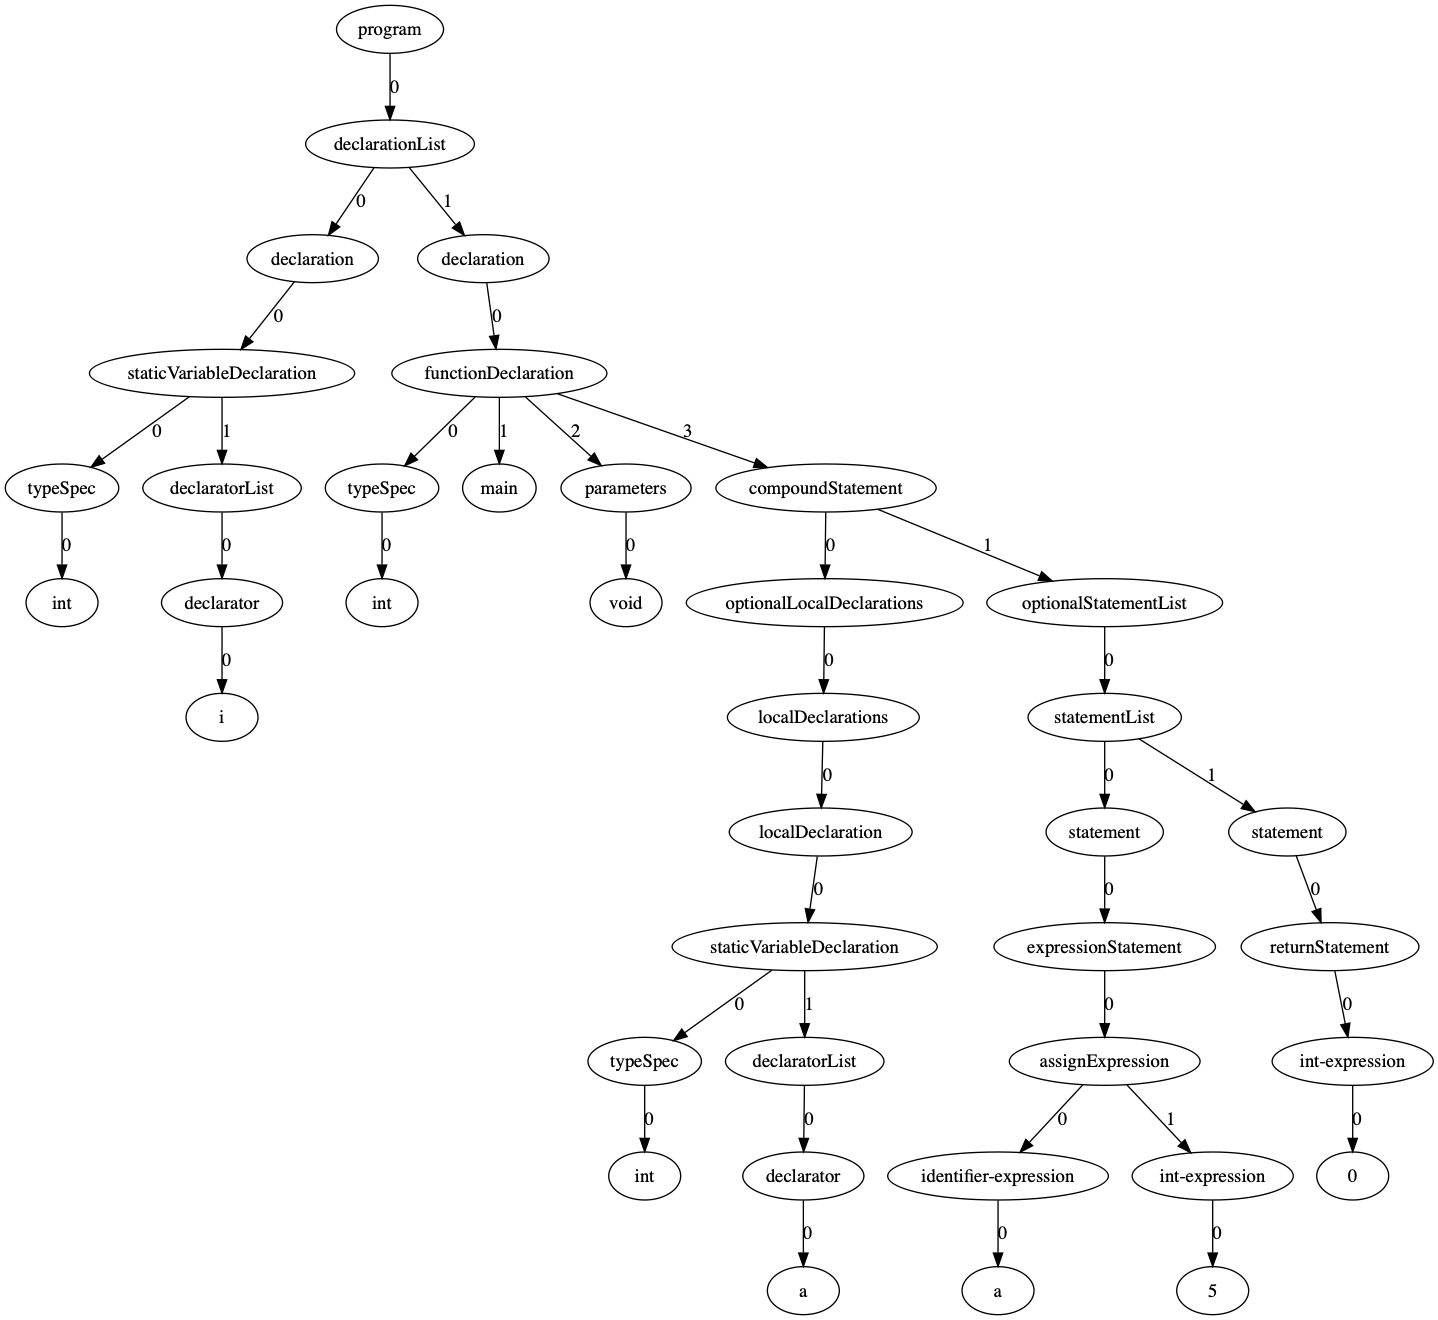
\includegraphics[width=\linewidth]{img/tree.png}
\end{figure}
\subsection{错误处理}

\subsubsection{语法错误的处理}

\quad\ \ 主要通过yacc的error处理函数实现,当检测到不在定义中的语法规则时,yacc自动调用p\_error函数,并以当前处理的token作为参数。

\begin{minted}{python}

def p_error(p):
       print('Syntax Error occur around', 'line:', p.lineno)
       print('Syntax Error occur around', p.type,':', p.value)
       exit()

\end{minted}

上述语法错误处理函数将token中记录的当前行号lineno和处理到的符号类型type和值value进行格式化打印,并调用exit()结束语法分析。

\subsubsection{语义错误的处理}

\quad\ \ 由于我们采用了中间代码生成和语义分析一起处理的方法,语义错误的处理在生成中间代码的过程中处理错误。

具体做法是在分析的过程中通过Python的assert函数指明当前必须满足的条件,并在条件不满足时执行相应的错误处理函数。

例如,下面的find\_addr函数是语义分析和中间代码生成过程中寻找变量地址的函数。当表达式既不在当前局部变量表和局部参数表中,也不在全局变量表中时,打印一个语义错误信息,并抛出错误。这意味着在当前环境下使用的该变量没有声明。

\begin{minted}{python}

def find_addr(expression):
       if type(expression)!=str:
            return (None,None,None)
       global local_var,local_para,global_var
       for i in range(len(local_var)):
             if local_var[i][1]==expression:
                  return (False,local_var[i][0],local_var[i][3])
       for i in range(len(local_para)):
             if local_para[i][1]==expression:
                  return (False,local_para[i][0],local_para[i][3])
       for _ in global_var:
             if _[1]==expression:
                  return (True,_[0],None) 
       print('Semantic Error: Cannot find address for expression:', expression)
       assert(False)

\end{minted}

\subsubsection{语法错误测试结果}

\begin{minted}{c}
int i;

int main(void)
{
    int a, b
    a = 0;
    b = 2;
    for(i=0;i<10;i=i+1){
    a = a + b;
}
    printf("%d\n", a);
    return 0;
}
\end{minted}

\begin{minted}{shell}
Syntax Error occur around line: 6
Syntax Error occur around ID : a
\end{minted}

\subsubsection{语义错误测试}

\begin{minted}{c}
int i;

int main(void)
{
    int a, b;
    a = 0;
    b = 2;
    for(i=0;i<10;i=i+1){
        a = a + c;
    }
    printf("%d\n", a);
    return 0;
}
\end{minted}

\begin{minted}{shell}
main proc
local_para = []
(':=', 0, None, ('a', (False, 'int', -8)))
(':=', 2, None, ('b', (False, 'int', -4)))
(':=', 0, None, ('i', (True, 'int', None)))
main_L1:
('<', ('i', (True, 'int', None)), 10, ('temp_var_4', (True, 'int', 0)))
('j==', ('temp_var_4', (True, 'int', 0)), 0, 'main_L2')
Semantic Error: Cannot find address for expression: c
\end{minted}

上述结果表明在中间代码生成的过程中发现了错误。


\end{document}